\section{Логическое проектирование}

\subsection{Построение логической концептуальной модели данных}

Нас основе этапов инфологического проектирования построим логическую концептуальную модель согласно методологии IDEF1X.\par 

\begin{figure}[h!]
    \centering
    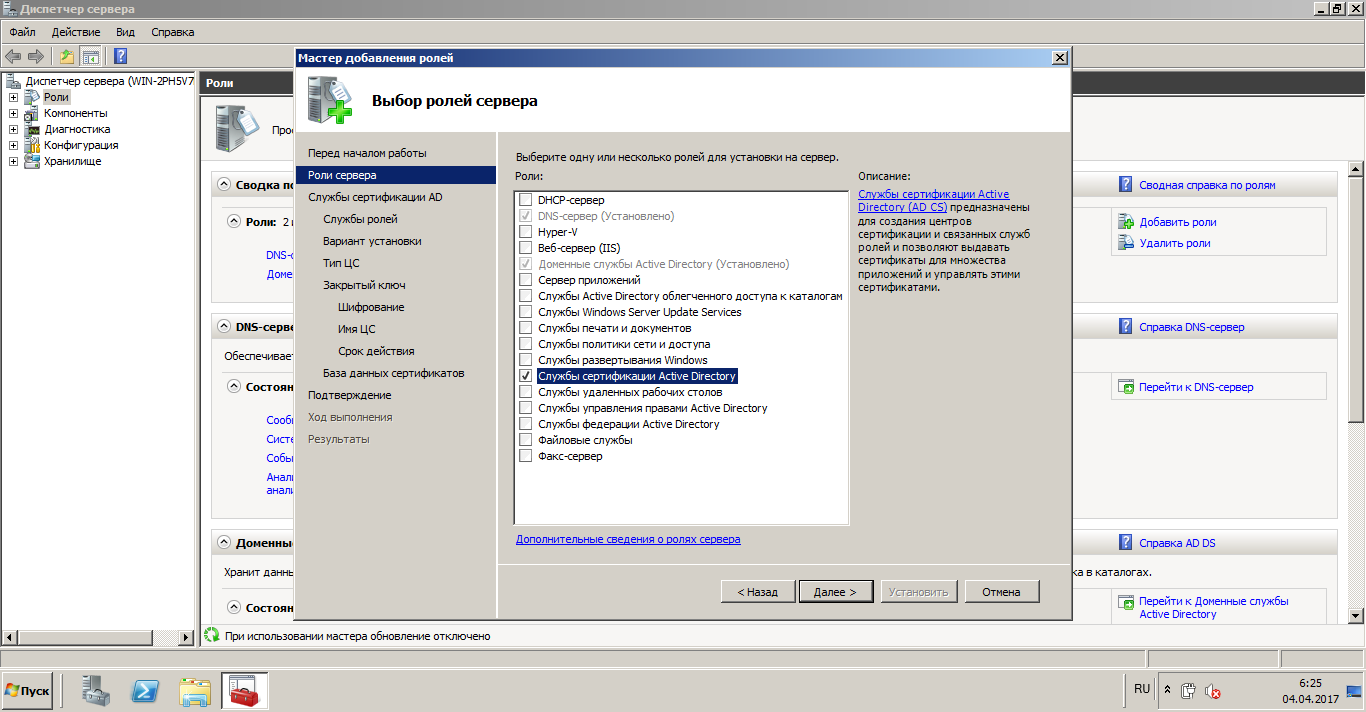
\includegraphics[width=0.7\textwidth]{3}
    \caption{Логическая концептуальная модель данных}
    \label{img:3}
\end{figure}

\vspace{0.8cm}

\clearpage

\subsection{Определение функциональных зависимостей}

\begin{itemize}
\item f: CAR\_TYPES, uid (PK) - car\_type;
\item f: STATIONS, uid (PK) - name;
\item f: ROUTES, uid (PK) - first\_station (FK), last\_station (FK), num;
\item f: TRIPS, uid (PK) - route (FK), start\_dt, end\_dt;
\item f: CARS, uid (PK) - trip (FK), num, car\_type (FK), places;
\item f: PLACES, uid (PK) - car (FK), num, is\_upper, price, is\_bought.
\end{itemize}

\vspace{0.8cm}

\subsection{Составление реляционных таблиц}

    Ограничения на поля таблиц:
    \begin{itemize}
        \item в таблице ROUTES значение поля first\_station должно быть отличным от значения поля last\_station;
        \item в таблице CAR\_TYPES значение поля car\_type должно быть уникальным;
        \item в таблице ROUTES значение поля num должно быть уникальным и положительным;
        \item в таблице CARS значение поля num должно быть уникальным и положительным;
        \item в таблице CARS значение поля places должно быть положительным;
        \item в таблице PLACES значение поля num должно быть уникальным и положительным;
        \item в таблице CARS значение поля price должно быть положительным;
        \item ни в одной таблице ни одно поле не должно быть пустым.
    \end{itemize}
    
    Значения по умолчанию:
    \begin{itemize}
        \item в таблице STATIONS значение поля name по умолчанию - 'Томск';
        \item в таблице TRIPS значение поля start\_dt по умолчанию - текущая дата-время по UTC;
        \item в таблице TRIPS значение поля end\_dt по умолчанию - текущая дата-время по UTC;
        \item в таблице CAR\_TYPES значение поля car\_type по умолчанию - 'Плацкарт';
        \item в таблице CAR значение поля num по умолчанию - 1;
        \item в таблице PLACES значение поля num по умолчанию - 1;
        \item в таблице PLACES значение поля is\_upper по умолчанию - FALSE;
        \item в таблице PLACES значение поля price по умолчанию - 1;
        \item в таблице PLACES значение поля is\_bought по умолчанию - FALSE.
    \end{itemize}
    
    Полученная схема данных представлена на рис. \ref{img:01}.\par
    
    \begin{figure}[h!]
        \centering
        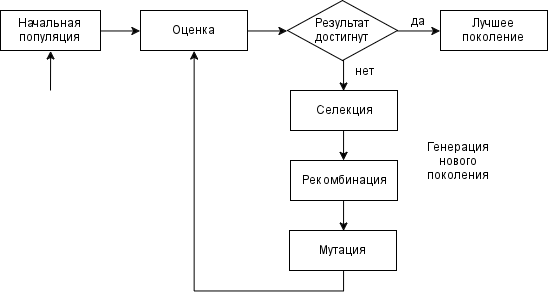
\includegraphics[width=0.7\textwidth]{4}
        \caption{Схема данных}
        \label{img:3}
    \end{figure}

    Таблицы БД находятся в первой нормальной форме, т.к. все значения полей таблиц CAR\_TYPES, CARS, ROUTES, STATIONS, PLACES и TRIPS являются атомарными, а все записи в этих таблицах являются уникальными.\par
    Таблицы БД находятся во второй нормальной форме, т.к. неключевые поля таблиц CAR\_TYPES, CARS, ROUTES, STATIONS, PLACES и TRIPS полностью зависят от всего первичного ключа uid.\par
    Таблицы БД находятся в третьей нормальной форме, т.к. все неключевые поля таблиц CAR\_TYPES, CARS, ROUTES, STATIONS, PLACES и TRIPS зависят только от первичного ключа.\par
    
    \vspace{0.8cm}
    
    \subsection{Глоссарий}
        В глоссарии приведены следующие формальные определения имён таблиц и атрибутов:
        \begin{itemize}
            \item STATIONS - таблица со станциями;
            \item ROUTES - таблица с маршрутами следования;
            \item TRIPS - таблица с рейсами поездов;
            \item CAR\_TYPES - таблица с видами вагонов;
            \item CARS - таблица с вагонами поездов;
            \item PLACES - таблица с местами вагонов поездов;
            \item uid - уникальный идентификатор, целое положительное число с автоинкрементом, не пустое поле;
            \item name - название станции, текст, не пустое поле;
            \item first\_station (FK) - станция отправления маршрута, внешний ключ, целое положительное число, не пустое поле;
            \item last\_station (FK) - станция прибытия маршрута, внешний ключ, целое положительное число, не пустое поле;
            \item num - номер рейса, целое положительное число, не пустое поле;
            \item route (FK) - маршрут рейса, внешний ключ, целое положительное число, не пустое поле;
            \item start\_dt - дата-время отправления рейса, дата-время, не пустое поле;
            \item end\_dt - дата-время прибытия рейса, дата-время, не пустое поле;
            \item car\_type - вид вагона, целое положительное число, не пустое поле;
            \item trip (FK) - рейс вагона, внешний ключ, целое положительное число, не пустое поле;
            \item num - номер вагона, целое положительное число, не пустое поле;
            \item car\_type (FK) - тип вагона, внешний ключ, целое положительное число, не пустое поле;
            \item places - количество мест в вагоне, целое положительное число, не пустое поле;
            \item car\_type - тип вагона, текст, не пустое поле;
            \item car (FK) - вагон места, внешний ключ, целое положительное число, не пустое поле;
            \item num - номер места, целое положительное число, не пустое поле;
            \item is\_upper - флаг верхнего места, логическая переменная, не пустое поле;
            \item price - цена места, вещественное положительное число, не пустое поле;
            \item is\_bought - флаг купленного места, логическая переменная, не пустое поле. 
        \end{itemize}

\clearpage